% !TEX encoding = UTF-8
% !TEX program = pdflatex
% !TEX root = InformationRetrieval.tex
% !TEX spellcheck = it-IT

% 30 Settembre 2016
% \chapter{Introduzione}
% \section{Programma e quadro d'insieme}
% \subsection{Programma}

\subsection{Indicizzazione}

\begin{figure}
	\centering
	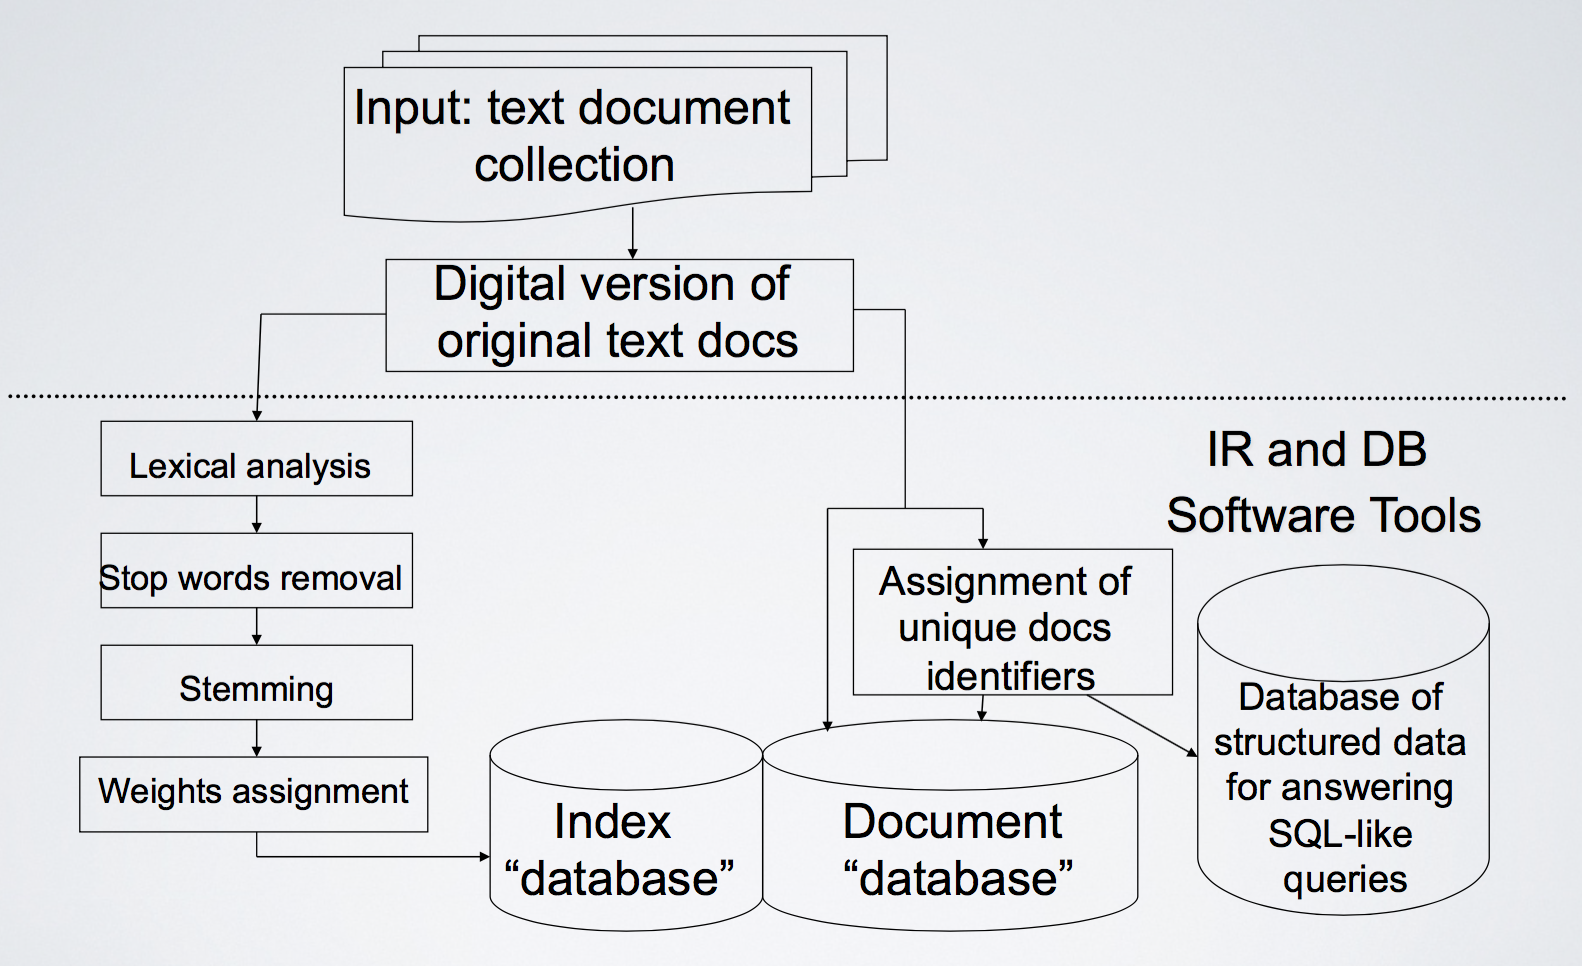
\includegraphics[width=0.6\textwidth]{images/l2-indicizzazione.png}
	\caption{Indicizzazione dei documenti}
\end{figure}

Si parte da un insieme di documenti in un qualche formato digitale che devono essere opportunamente trasformati in formato testuale, per poi effettuare una sorta di analisi lessicale.
In parallelo all'analisi del documento è necessario andare ad assegnare un identificativo ad ogni documento. Si ha quindi che la coppia ``documento processato/identificatore'' vanno a creare la nostra base di dati.

Tipicamente nella base di dati viene conservata sia la versione originale del documento, in modo da poterla fornire all'utente, che la versione processata.

Ovviamente finché non sono stati indicizzati tutti i documenti, non è possibile rispondere alle query, ma una volta terminata l'indicizzazione è sempre possibile andare ad estendere la base di dati, indicizzando nuovi documenti.

\`E inoltre possibile estendere la base di dati in modo che contenga anche dei dati strutturati che descrivono i documenti, in modo da poter rispondere in modo efficiente e deterministico alle query specifiche del tipo \textit{``tutti i documenti scritti da Pippo''}.

Un'altra cosa fondamentale è l'\textbf{autorevolezza} della collezione dei documenti, ovvero è necessario discriminare e dare importanza diversa a documenti che provengono da fonti diverse. Ad esempio se si vogliono reperire delle informazioni riguardo una certa tematica è necessario dare maggiore importanza a quelle fonti ritenuti autorevoli rispetto quella tematica e meno alle informazioni reperite dalle pagine web generiche.

Si ha quindi che una delle parti principali di un sistema di reperimento dell'informazione è la creazione dell'\textbf{index} dei documenti, il quale viene spesso chiamato \textbf{inverted index} (indice trasposto) perché permette di risalire ai documenti a partire dalle parole in esse contenute. 
Questo indice deve essere molto dettagliato e quindi l'ordine di grandezza della dimensione dell'indice è paragonabile a quello della collezione dei documenti.

\subsection{Reperimento}

\begin{figure}
	\centering
	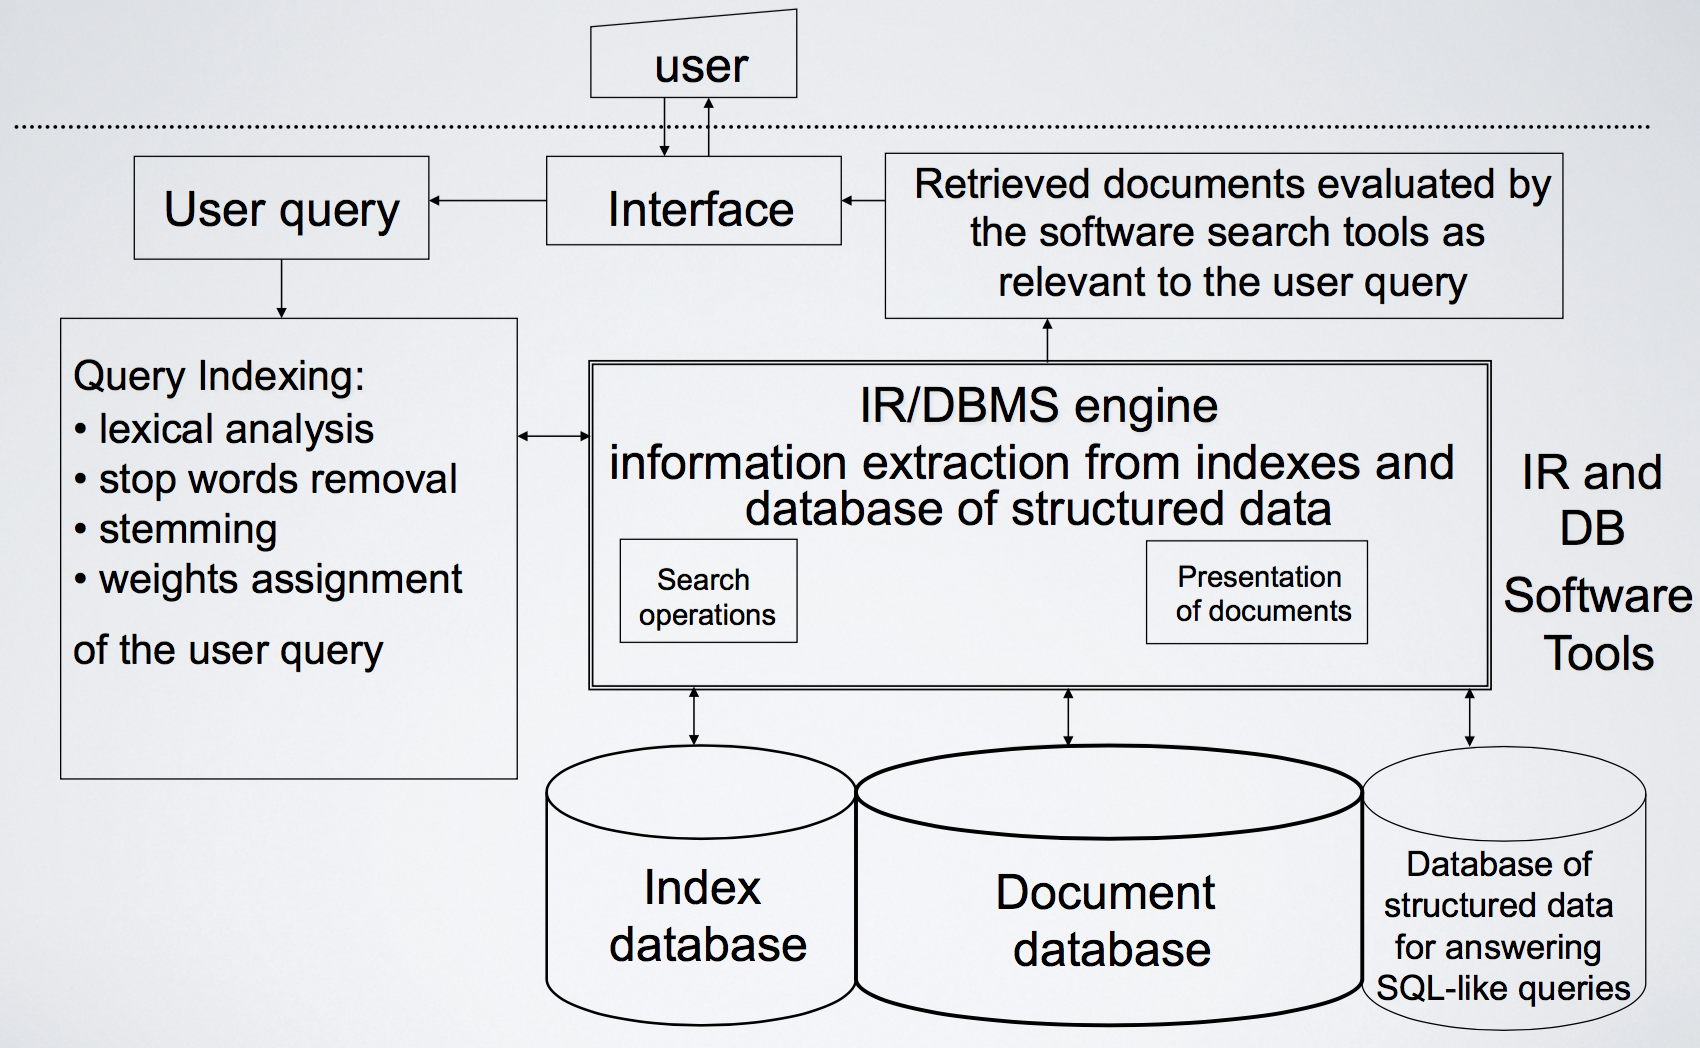
\includegraphics[width=0.6\textwidth]{images/l2-reperimento.png}
	\caption{Reperimento dell'informazione}
\end{figure}

Tutto inizia dall'utente che esprime in linguaggio naturale o in modo semplificato la query attraverso una qualche interfaccia che non è necessariamente via web. Questa query deve essere processata in modo analogo ai documenti nella fase di indicizzazione.

La ricerca viene poi effettuata in base alla query, perché in alcuni casi è necessario andare a fare reperimento dell'informazione, mentre in altri casi è possibile utilizzare l'approccio \textit{SQL-Like}.

Una volta trovati i documenti relativi alla query, questi vengono inviati all'utente ordinati per rilevanza rispetto alla query effettuata.

Ci sono poi delle differenze se il sistema lavora con documenti presenti nel web, perché in primo luogo non è necessario creare un identificatore per i documenti dato che è possibile utilizzare un URL.
Inoltre, è necessario scegliere quali informazioni del documento mantenere memorizzate all'interno della base di dati. Ad esempio si può scegliere di mantenere solamente i meta-dati della pagina\footnote{tipicamente viene tenuta la data dell'ultimo aggiornamento, in modo da riuscire a capire se l'indice è diventato obsoleto.} e non tutto il documento, che tanto può essere facilmente reperito tramite l'URL.

Il bisogno dell'utente viene chiamato \textbf{esigenza informativa} o \textbf{topic}, mentre la \textbf{query} è la rappresentazione dell'esigenza informativa dell'utente.
Da notare che la query può essere incompleta perché l'utente può non conoscere nel dettaglio la sua esigenza informativa oppure non riesce ad esprimere al query con l'interfaccia fornita.

C'è poi una distinzione tra \textbf{termine} e \textbf{parola}. Un termine può presentarsi sotto varie forme, in base a come deve essere espressa la query: \textit{date, frasi, numeri, espressioni regolari, ecc.} mentre una parola è una parola in senso letterale.
Tipicamente è anche possibile utilizzare una \textbf{wildcard} per indicare che si vuole fare un match parziale su una determinata parola.

Si riesce quindi a fornire all'utente un \textbf{query language} molto complesso che permette di applicare dei filtri per restringere l'insieme di ricerca. Tuttavia l'utente tipo si limita ad esprimere la query utilizzando solamente delle semplici parole.

Un \textbf{motore di ricerca} è quindi un sistema di reperimento dell'informazione che opera su una macchina locale o su un sistema distribuito, utilizzando le informazioni presenti nell'inverted index.

Il risultato dell'operazione di reperimento è la lista ordinata di documenti (\textbf{relevance ranking}) secondo un \textbf{retrieval status value}.
L'ordinamento di questa lista è uno dei problemi fondamentali del reperimento dell'informazione.

\begin{figure}[htbp]
	\centering
	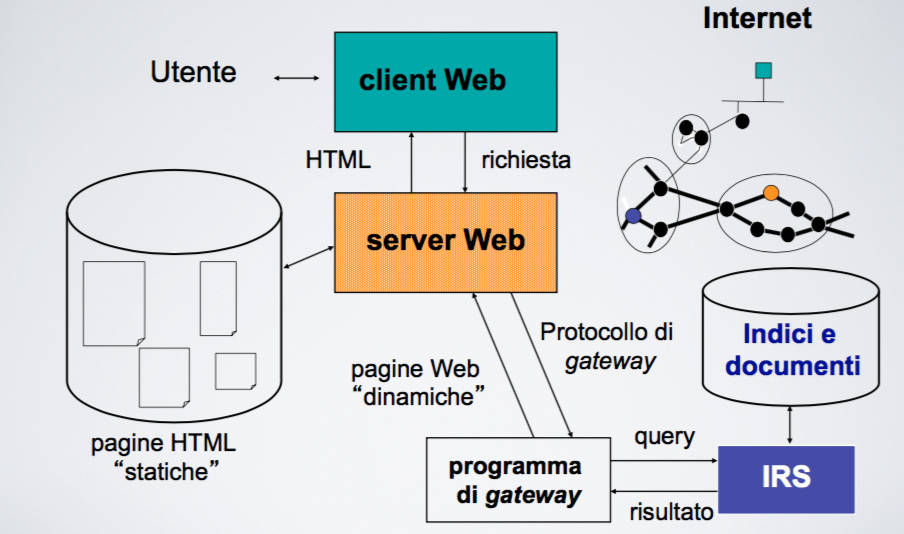
\includegraphics[width=.6\textwidth]{images/l2-irsweb.png}
	\caption{Accesso ad un IRS tramite un client web}
\end{figure}

\subsection{Valutazione delle prestazioni}

Ci sono due aspetti principali da valutare:

\begin{itemize}
	\item \textbf{Efficienza}: riguarda il tempo necessario a fornire una risposta, allo spazio occupato dalla base di dati, ecc. In modo molto simile a quello che viene fatto nell'Ingegneria del Software.
	\item \textbf{Efficacia}: riguarda la \textbf{rilevanza} dei risultati prodotti rispetto l'esigenza informativa dell'utente. Risulta più difficile da valutare perché dipende dal giudizio dell'utente, il quale a sua volta dipende da quanto l'utente conosce riguardo l'argomento che sta cercando, da quanto bravo è ad esprimere la query e da quanto è in grado di valutare la pertinenza dei documenti ritrovati.
\end{itemize}

\chapter{Rappresentazione dei documenti}

Per recuperare dei documenti di interesse, prima di tutto occorre rappresentare il \textbf{contenuto informativo} del documento.
Serve quindi un sistema che sia in grado di effettuare un'analisi del testo in modo automatico, rapido, affidabile e consistente in modo da riuscire ad ottenere la maggior quantità possibile di informazioni.
Questo vale anche per i documenti che sono già in formato testuale.

\section{Analisi automatica del testo}

Per analizzare il testo ci sono due tipologie principali di approcci

\begin{itemize}
	\item \textbf{Statistico}: quello che affronteremo noi e che si basa sull'utilizzo di regole matematiche, come il conto delle occorrenze di un termine. Il pioniere di questo approccio è stato Hans Peter \textbf{Luhn}, secondo il quale {\color{Red}le frequenze con le quali le parole appaiono in un testo possono essere utilizzate per selezionare le parole e le frasi utili a rappresentare il contenuto di un testo}, ovvero la distribuzione di frequenza delle parole in un testo non è uniforme, ci sono poche parole molto frequenti e tante parole poco frequenti. Queste ultime sono quelle che giocano un ruolo chiave nella creazione dell'indice.
	\item \textbf{Linguistico}: richiede elevate competenze linguistiche per ottenere risultati migliori, ma dal punto di vista informatico questo risulta più difficile da applicare.
\end{itemize}
